\documentclass{article} % For LaTeX2e
\usepackage{nips15submit_e,times}
\usepackage{hyperref}
\usepackage{url}
%\documentstyle[nips14submit_09,times,art10]{article} % For LaTeX 2.09

\usepackage{graphicx}
\usepackage{subfigure}
\usepackage{algorithmic}
\usepackage{algorithm}
\usepackage{amsmath}
\usepackage{multirow}
\usepackage{amssymb}
% \usepackage{wrapfig,lipsum,booktabs}
\usepackage{wrapfig}

%\usepackage{etoolbox}
%\patchcmd{\thebibliography}{\section*{\refname}}{}{}{}

\title{Clustering Gamers's Time Series Data : A Case Study}

\author{
Yuanli Pei\thanks{This work was done while Yuanli Pei and Moises Goldszmidt were at Zynga Inc.} \\
Oregon State University, Corvallis, OR\\
\texttt{peiy@eecs.oregonstate.edu} \\
\And
Amy Tan\\
Zynga Inc, San Francisco, CA\\
\texttt{atan@zynga.com} \\
\AND
Moises Goldszmidt$^\ast$ \\
Affiliation, Address \\
\texttt{moises.goldszmidt@gmail.com} \\
\And
Alexandros Ntoulas\\
Zynga Inc, San Francsico, CA \\
\texttt{antoulas@zynga.com} 
}


% \author{
% David S.~Hippocampus\thanks{ Use footnote for providing further information
% about author (webpage, alternative address)---\emph{not} for acknowledging
% funding agencies.} \\
% Department of Computer Science\\
% Cranberry-Lemon University\\
% Pittsburgh, PA 15213 \\
% \texttt{hippo@cs.cranberry-lemon.edu} \\
% \And
% Coauthor \\
% Affiliation \\
% Address \\
% \texttt{email} \\
% \AND
% Coauthor \\
% Affiliation \\
% Address \\
% \texttt{email} \\
% \And
% Coauthor \\
% Affiliation \\
% Address \\
% \texttt{email} \\
% \And
% Coauthor \\
% Affiliation \\
% Address \\
% \texttt{email} \\
% (if needed)\\
% }

% The \author macro works with any number of authors. There are two commands
% used to separate the names and addresses of multiple authors: \And and \AND.
%
% Using \And between authors leaves it to \LaTeX{} to determine where to break
% the lines. Using \AND forces a linebreak at that point. So, if \LaTeX{}
% puts 3 of 4 authors names on the first line, and the last on the second
% line, try using \AND instead of \And before the third author name.

\newcommand{\fix}{\marginpar{FIX}}
\newcommand{\new}{\marginpar{NEW}}

\nipsfinalcopy % Uncomment for camera-ready version

\begin{document}


\maketitle

\begin{abstract}
Game industry plays an important in improving our entertainment in digital life. 
One of the main tasks for the game companies is to develop user-specific features to 
improve their gaming experience. The key factor is to understand player's behaviors during their 
game-play. This paper  considers the following two tasks: 
Given user's time series behavior data, 1) what are the underlying playing states that 
controls user's behaviors at each time period, and 2) what are the natural groups of players based 
on their state transitions. We apply Hidden Markov Model (HMM) to identify gamers' 
hidden playing states, and use a Dirichlet clustering method to find player groups based on 
their state transitions. Our case study on one of the strategy game developed by Zynga Inc.\  
reveals interesting results that can help gamer designers to improve the game.


\end{abstract}


\section{Introduction}
As game industry immerses, playing games has become an important entertainment activity in our digital life. 
To improve players' experience, it is very important for game companies to understand 
player's behaviors and design user-specific features. As players may change their playing strategies 
during the game-play, understanding gamer's playing pattens over time becomes an important task. 

In this paper, we study the problem of understanding users' behaviors from their time series data obtained
during the game-play.  In particular, we focus on two tasks: 
1) what are the underlying playing states that controls user's behavior at each time period, 
and 2) what are the natural groups of players based on their state transitions (game playing strategy). 
We model user's time series data using Hidden Markov Model (HMM) \cite{hmm}, with the playing states as 
the hidden nodes and the players' statistics at each time period as the observed features. 
We fit the HMM model and find users' playing states by applying Viterbi decoding algorithm. 
We then find the groups of players using an unsupervised Dirichlet clustering method.

We experiment our method on a mobile strategy game developed by Zynga Inc. %, named {\it Empires and Allies}. 
Our method found three underlying playing states, and  the clustering results reveal three 
interesting groups that contains players with similar transition states within each group.
All these results are helpful to understanding players' behaviors and improve the game design. 




\section{Related Work}
To do.


\section{Method}
Let $X_{it} = [X_{it1}, \cdots, X_{itD}]^\top$ be the measurements of player $i$ at the $t$-th time period, 
where $D$ is the number of features. Suppose we have the measurements of player $i$ from $1$ to the 
$T$-th time period\footnote{Note that for different users, the total time periods are not necessarily the same. 
Here for simplicity we assume that all users are measured during the same amount of time},
denoted as $X_{i} = [X_{i1}, \cdots, X_{iT}]^\top$. For a total number of $N$ players, we have their time series 
data $X = \{ X_1, \cdots, X_N \}$.

Our method includes two steps corresponding to the two tasks: 1) using HMM model to identify gamers' 
playing states at each time period, and 2) discovering player groups based on their transitions over states by clustering. 
Below we describe these two steps in detail.

\subsection{Identify Gamers' Playing States Using HMM Model}
We assume that there is an underlying playing state that controls
user’s behaviors at each time period, and the state evolves  as the player changes his strategy over
time. We represent each gamers' data using a Hidden Markov Model (HMM) \cite{hmm} chain with 
length $T$, the total time periods.  Let $Y_{it}$ be the hidden state representing 
the $i$-th gamer's underlying playing state at time $t$, and $Y_{it}$ is discrete which can take on $S$ values $\{1, \cdots, S\}$.

%The gamer's HMM model has three parameters: 1) the initial state distribution vector $\pi$ 
%with $\pi_s$ being the probability of a gamer starting with state $s$; 
%2) the state transition parameter $A$, with $A_{rs}$ being the probability of a gamer transitioning from state
%$r$ at time $t-1$ to state $s$ at time $t$. 3) the emission parameter $B$, with $B_s$ controlling the probability of observing $X_{it}$ at state $Y_{it} = s$. 

The mechanism of the gamers' HMM model is as below: 1) initially, a gamer starts with state 
$Y_{i1} \in \{1, \cdots, S\}$ according to an initial distribution $\pi$,  with $\pi_s$ being 
the probability of starting at state $s$; 2) all the $Y_{it}$'s  evolves according to the 
{\it Markov property}: given $Y_{i{t-1}}$, the state $Y_{it}$ is independent of all the 
states prior to $t-1$, and the transition matrix is $A$, with $A_{rs}$ being the probability of 
transitioning from state $r$ to state $t$; 3) at each time $t$, the observations $X_{it}$ only 
depends on the state $Y_{it}$ parametrized by $B$, with $B_s$ controlling the probability 
of observing $X_{it}$ at state $Y_{it} = s$. 


Given the observed data $X$ and the number of states $S$, we can estimate the parameters by maximizing the 
likelihood of the observations
\[
  \max_{\pi, A, B} P(X | \pi, A, B)
= \prod_{i=1}^N P(Y_{i1} | \pi) P(X_{i1} | Y_{i1}, B)
  \prod_{t=2}^T P(Y_{it} | Y_{i{t-1}}, A) P(X_{it} | Y_{it}, B) ~.
\]
However, in the application of modeling gamers' playing states, the number of states $S$ is usually unknown. 
We will estimate $S$ using criteria such as changes of data likelihood, AIC or BIC. 
 
After estimating the parameters, the state sequence $Y_{i1}, \cdots, Y_{iT}$ 
for each user can be found using Viterbi decoding \cite{hmm} which maximizes
$P(Y_{i1}, \cdots, Y_{iT}| X, \pi, A, B)$. 
%One possible solution is to estimate $Y_{it}$ individually by maximizing $P(Y_{it}| X_{it}, \pi, A, B)$.

\subsection{Clustering Gamers based on State Transitions}
\label{sec:clustering}
The next step is to clustering the gamers based on their trends of state transitions. 
Here we adopt a similar method that has been successfully applied to crisis identification in distributed computing system \cite{moises}. 
Let $Y = [Y_1, \cdots, Y_N]^\top$ be the state transitions for all the players,
where $Y_i = [Y_{i1}, \cdots, Y_{iT}]^\top$ denotes the $i$-th player's states from 1 to
the $T$-th time. We denote $Z_i$ as the underlying cluster assignment for the $i$-th player. 
Let $K$ be the total number of (unknown) clusters, which we will found automatically.

\subsubsection{The Clustering Model}
We adopt the mixture of Dirichlet process model (DP) for clustering \cite{dpclustering}. 
Suppose the clusters evolves according to a Dirichlet distribution with parameter $\alpha$.
We assume that each cluster $k$ generates a Markov chain parametrized by $\{\lambda^k, \Phi^k\}$, 
where $\lambda^k$ is the $S\time 1$ vector for the initial state distribution, 
and $\Phi^k$ is the $S \times S$ transition matrix. We use the prior distribution 
for parameters in each cluster is $G_0(\{\lambda^k, \Phi^k\}) = Dir(\hat\pi) \prod_{s=1}^S Dir (\hat B_{s.})$,
where $\hat\pi$ and $\hat B$ are the estimated parameters at the first step. 
The conditional probability  
\begin{equation}
\label{eq:condi}
  P(\{\lambda^k, \Phi^k \}_{k=1}^K | Z ) 
= \prod_k G_0(\{\lambda^k, \Phi^k\})~.
\end{equation}

%The data generation process is assumed as below \\
%\begin{tabular}{l}
%    \quad For each player $i$,\\
%    \qquad 1. Sample cluster assignment $Z_i \sim Dir(\alpha)$  \\
%    \qquad 2. Generate the state sequence $Y_{i1}, \cdots Y_{iT}$ with Markov chain parametrized by $\{\lambda^{Z_i}, \Phi^{Z_i}\}$.
%\end{tabular}
 

Given the clustering model, the likelihood of the data of state transitions for all players is
\begin{equation}
\label{eq:likeli}
  P(Y| Z, \{\lambda^k, \Phi^k \}_{k=1}^K) 
= \prod_{i=1}^N \left( \prod_{s=1}^S \lambda^{\mathbf{1}[Y_{i1} = s]} \prod_{r=1}^S \left(\Phi_{rs}^{Z_i}\right)^{n_{irs}} \right)~,
\end{equation}
where $\mathbf{1} [\cdot]$ is the indicator function, and $n_{irs}$ is the number of transitions from state $r$ to state $s$ for the $i$-th player.

\subsubsection{MCMC Sampling of Posterior Distribution}
Here we use a collapsed-space sampling method \cite{neal2000markov,collapsed_escobar} to obtain samples from the reduced-spaced posterior distribution $P(Z|Y)$, instead of the full-space distribution $P(Z, \{\lambda, \Phi\} | Y)$. This allows for easy sampling steps and faster convergence rate. 
The reduced-space posterior distribution is
\begin{equation*}
 P(Z|Y) \propto P(Z, Y) = P(Y|Z) P(Z).
\end{equation*}
The likelihood $P(Y|Z)$ can be computed by integrating out the cluster-specific parameters $\{\lambda^k, \Phi^k\}_{k=1}^K$.
Substituting  (\ref{eq:condi}) and (\ref{eq:likeli}), we obtain
%\begin{equation*}
%\renewcommand*{\arraystretch}{1.8}
%\begin{array}{rl}
%     P(Y|Z) 
%~ = & \int  P(Y| Z, \{\lambda^k, \Phi^k \}_{k=1}^K) P(\lambda^k, \Phi^k | Z) d\lambda^k d\Phi^{k} \\
%~ = & \displaystyle{ \prod_{k=1}^K 
%      \left[ 
%      \frac{\prod_s \Gamma(\hat \pi_s + \sum_{i} \mathbf{1}[Z_i=k,Y_{i1} = s]) \Gamma (\sum_s \hat \pi_s)}
%           {\Gamma\left( \sum_s (\hat  \pi_s + \sum_{i} \mathbf{1}[Z_i=k,Y_{i1} = s]) \right) \prod_s \Gamma (\hat \pi_s)}
%      \right]  } \times \\
% &  \displaystyle{ \prod_{k=1}^K \prod_r 
%      \left[ 
%      \frac{\prod_s \Gamma(\hat B_{rs} + \sum_{i} \mathbf{1}[Z_i=k] n_{irs} ) \Gamma (\sum_s \hat B_{rs})}
%           {\Gamma\left( \sum_s (\hat  B_{rs} + \sum_{i}\mathbf{1}[Z_i=k]  n_{irs} ) \right) \prod_s \Gamma (\hat B_{rs})}
%      \right] } ~,
%\end{array}
%\end{equation*}
\begin{equation*}
\renewcommand*{\arraystretch}{1.9}
\begin{array}{rl}
     P(Y|Z) 
~ = & \int  P(Y| Z, \{\lambda^k, \Phi^k \}_{k=1}^K) P(\lambda^k, \Phi^k | Z) d\lambda^k d\Phi^{k} \\
~ = & \displaystyle{ \prod_{k=1}^K 
      \left[ 
      \frac{\prod_s \Gamma(\bar \pi_s) \Gamma (\sum_s \hat \pi_s)}
           {\Gamma\left( \sum_s \bar \pi_s \right) \prod_s \Gamma (\hat \pi_s)}
      \right]  } \times
    \displaystyle{ \prod_{k=1}^K \prod_r 
      \left[ 
      \frac{\prod_s \Gamma(\bar B_{rs}) \Gamma (\sum_s \hat B_{rs})}
           {\Gamma\left( \sum_s \bar  B_{rs} \right) \prod_s \Gamma (\hat B_{rs})}
      \right] } ~,
\end{array}
\end{equation*}
where
$\bar \pi _s = \hat \pi_s + \sum_{i} \mathbf{1}[Z_i=k,Y_{i1} = s]$, and
$\bar B_{rs} = \hat B_{rs} + \sum_{i} n_{irs}  \cdot \mathbf{1}[Z_i=k]$.

Sampling $Z$ from Dirichlet distribution can be equivalently done as below \cite{neal2000markov}: 
set $Z_1 = 1$; for subsequent players, sample $Z_i$ according to  the following distribution 
\begin{equation*}
\label{eq:condition}
\renewcommand*{\arraystretch}{1.5}
\begin{array}{rl}
    P(Z_i = k | Z_1, \cdots, Z_{i-1}) 
~~=& \frac{|\{i' < i : Z_{i'} = k\}|}{i-1 + \alpha}  ~, \quad \text{for } k \in \{Z_{i'}\}_{i' < i}  \\
   P(Z_i = Z_{i'}, \forall i' < i | Z_1, \cdots, Z_{i-1}) 
~~=& \frac{\alpha}{i-1 + \alpha} ~,
\end{array}
\end{equation*}
where $|\cdot|$ denotes the number of elements in a set.

Note that our clustering method can be easily extended to incorporate side information 
such as pairwise constraints \cite{constraintBook}, by only considering the samples $Z$ that
satisfying the constraints.



\section{Experiments}
We apply our method to Zynga Inc's strategy game called ``Empires and Allies''.
In the game, the goal is to conquer all the battlefields
in a global map,  either with machine or with other players. To conquer 
the battles, the players need to build/upgrade base resources such as weapons and troops, which in turn 
requires game points that can be obtained from winning battles.  Thus, the players need to 
tradeoff between building resources and conquering battlefields.

%We apply our method to one of Zynga Inc's mobile strategy game -- Empires and Allies, an all-new modern military strategy game that players can design their army, build their base and deploy their weapons and troops to conquer the battlefields. Thanks to the powerful backend system, the game tracks almost every action each player does in the game, which provide us a handful data set to investigate the sophisticated player types. We choose a data set which contains a daily active cohort's 10 consecutive days data from the first day they install the game. For each player and each day, we have 67 features including engagement features like session length, number of battles, game action features like deploy a tank, build a defence building and join an alliance. Then we use the feature selection algorithm to choose 5 out of 67 features to build the time series clustering model. They are PvP (People vs People) Battle , PvE (People vs Bot) Battle, Points gained/lost per battle, session length, Level up and is-Payer.  

We form a dataset that contains player's 10 consecutive days data after installation, 
and subsample users that are active at all the 10 days. This results in 1719 players.
Each player is measured with $67$ metrics at each day, and we select $5$ important 
features based on prior experience: \texttt{PvP} (people vs people battle), 
\texttt{Pve} (people vs machine battle), \texttt{Points} (number of points gained), \texttt{Session} 
(number of session started), \texttt{LevelUp} (whether a player level up) and \texttt{isPayer} (whether
the player paid). We model \texttt{Points}  with Gaussian distribution, \texttt{Session} with
Poisson distribution, and the rest features with Bernoulli distribution.


%\begin{wrapfigure}{r}{0.4\textwidth}
%\centering
%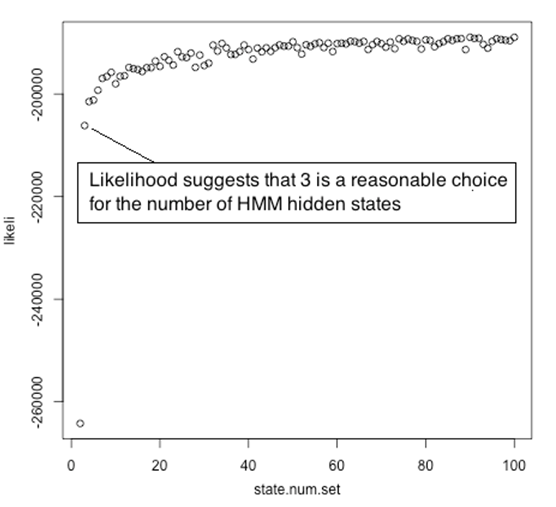
\includegraphics[width=0.35\textwidth]{likeli} 
%\caption{Data likelihood using different number of playing states.}
%\label{fig:likeli}
%\end{wrapfigure}




\subsection{Identifying Players' Daily States}
We fit HMM model with different number of playing states and found that 3 states is reasonable. 
%Figure \ref{fig:likeli} plots the data likelihood using different number of playing states. 
%From the results, we see that using 3 hidden states is reasonable for explaining our data. 
Table \ref{tab:states} lists the discovered playing states, \textbf{Aggressive}, 
\textbf{Defensive}, and \textbf{Moderate}.  The \textbf{Aggressive} state captures 
the mode where the players focus on conquering battles, while the \textbf{Defensive} 
state describes the stage that they build the resources. The \textbf{Moderate} is a mixture
of the two. These states interestingly identified the design of the game explained previously,
namely, the players have to conquer battles and build resources intermittently in order to improve. 
\begin{wraptable}{r}{8.2cm}
\caption{Discovered Playing States}
\label{tab:states}
\centering
\begin{tabular}{lccc} 
\bf Feature / State & \textbf{Aggressive}  & \textbf{Defensive}  &  \textbf{Moderate} 
\\ \hline \\
 Prob.\ \texttt{Pvp}     &  0.2472  & 0.0295 &  0.0947  \\
 Prob.\ \texttt{Pve}     &  0.2430  & 0.0581 &  0.1044 \\
 Mean \texttt{Points} &  88.10   & 1238.36 &  476.22 \\
 Mean \texttt{Session}&  4.58    &  34.19  & 12.95 \\
 Prob.\ \texttt{LevelUp} &  0.1664  & 0.0177  & 0.0553 \\
 Prob.\ \texttt{Pay}     &  0.0031  & 0.0956  & 0.0320 \\
\end{tabular}
\end{wraptable}

We then decode player's  states at each day.
Figure \ref{fig:transitions} plots the transitions for all the users among the 10 days. 
The result shows that most of the users starts with the \textbf{Moderate} or \textbf{Defensive} state, 
and then gradually transition to the \textbf{Aggressive} state. 
This is also consistent with the game design since the players can not start with many battles at
the beginning due to the resources restriction, but they ultimately need to 
conquer all the battlefields.

\begin{figure}[h]
\begin{minipage}[b]{0.3\linewidth}
    \centering
    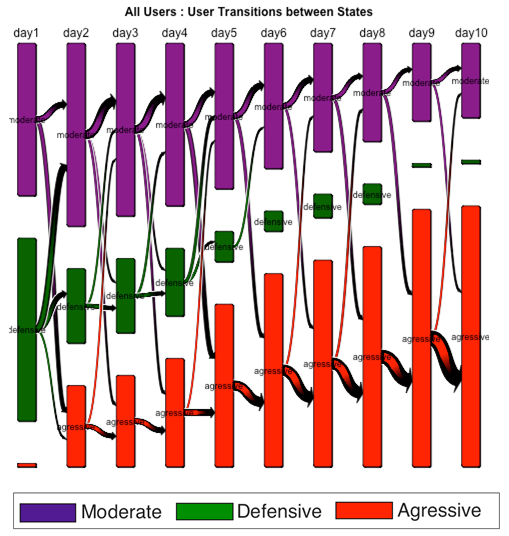
\includegraphics[width=0.8\linewidth]{transitions} 
    \caption{State transitions of all the Players at the first 10 days of installing the game.}
    \label{fig:transitions}
\end{minipage}
\quad
\begin{minipage}[b]{0.65\linewidth}
    \centering
        \begin{tabular}{ccc}
         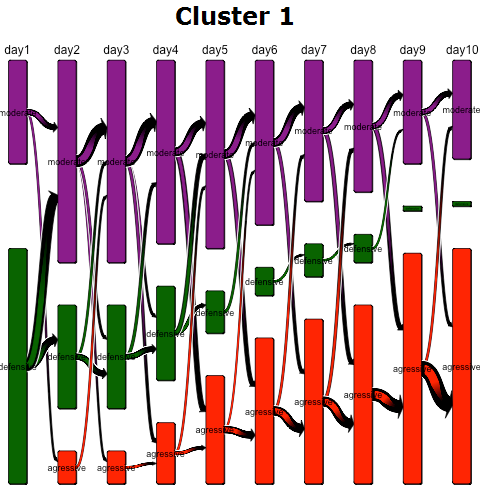
\includegraphics[width=0.33\textwidth]{cluster1} &
         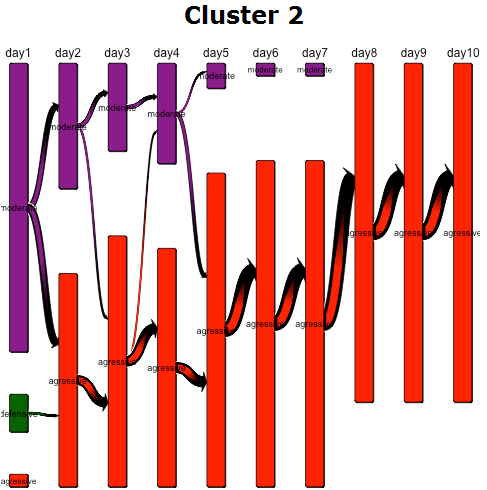
\includegraphics[width=0.33\textwidth]{cluster2} &
         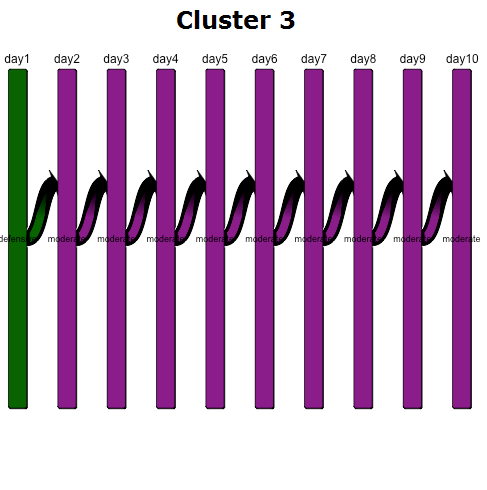
\includegraphics[width=0.33\textwidth]{cluster3} \\
         \multicolumn{3}{c}{ 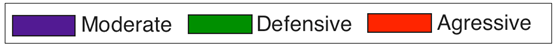
\includegraphics[width=0.8\textwidth]{legend} }
         \end{tabular}
     \caption{\label{fig:clusters} State transitions within three clusters found by our method.}
\end{minipage}
\end{figure}

%
%\begin{table}[t]
%\caption{Discovered Playing States}
%\label{tab:states}
%\centering
%\begin{tabular}{ccccccc}
%\bf State & \bf Pvp Pr. & \bf Pve Pr. & \bf Points Mean & \bf Session Mean & \bf LevelUp Pr. & \bf Pay Pr. 
%\\ \hline \\
%\texttt{Aggressive} & 0.2472  &  0.2430  &  88.10   &  4.58   & 0.1664  & 0.0031 \\  
%\texttt{Defensive}  & 0.0295  &  0.0581  &  1238.36 &  34.19  & 0.0177  & 0.0956 \\
%\texttt{Moderate}   & 0.0947  &  0.1044  &  476.22  &  12.95  & 0.0553  & 0.0320 
%\end{tabular}
%\end{table}


%\begin{figure}[t]
%\centering
%    \begin{tabular}{ccc}
%     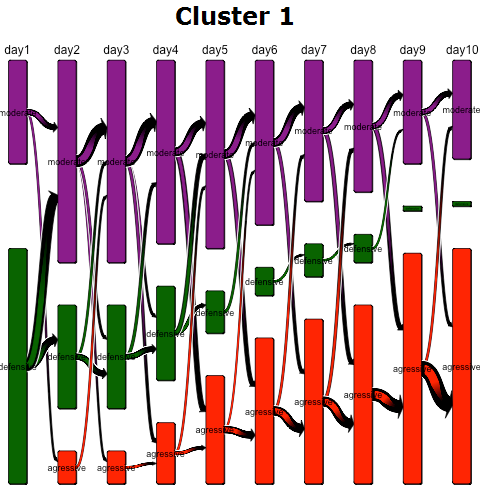
\includegraphics[width=0.26\textwidth]{cluster1} &
%     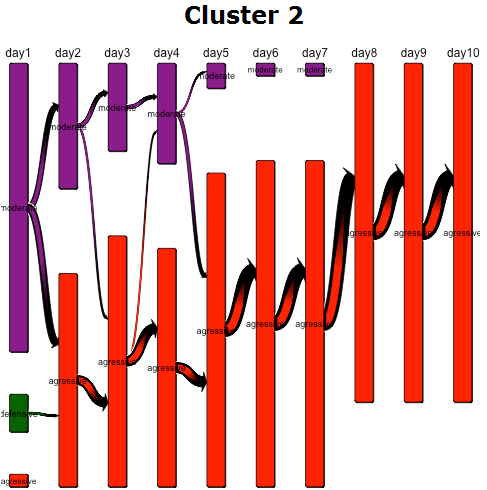
\includegraphics[width=0.26\textwidth]{cluster2} &
%     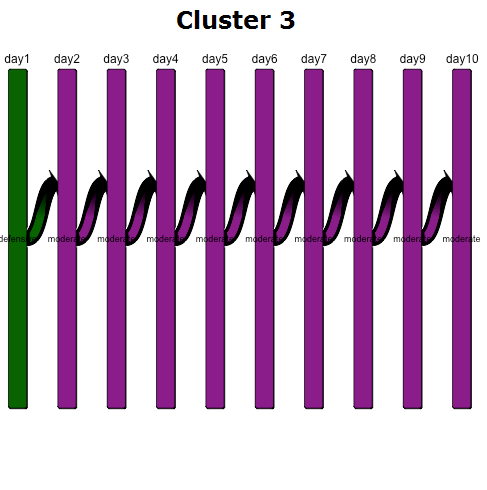
\includegraphics[width=0.26\textwidth]{cluster3} \\
%     \multicolumn{3}{c}
%      { 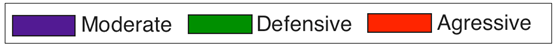
\includegraphics[width=0.45\textwidth]{legend} }
%    \end{tabular}
%     \caption{\label{fig:clusters} State transitions within the three clusters found by our method.
%              }
%\end{figure}
%
\subsection{Clustering Results}
Next we clustering users based on their state transitions with the method explained in Sec.\ \ref{sec:clustering} . 
\begin{wraptable}{r}{4.5cm}
\caption{Clustering results.}
\label{tab:clustering}
\begin{tabular}{ccc}
\bf Method & \bf \#Cluster & \bf DB
\\ \hline \\
{\bf Our}     & {\bf 3}  &  {\bf 0.968} \\  
Kmeans  &  5  &  2.628 \\
GMM     &  4  &  1.803 
\end{tabular}
\end{wraptable} 
We compare with two baselines: Kmeans and Gaussian Mixture Model (GMM). 
Due to the fact that we do not have actual cluster labels, we evaluate the results using a polular
internal evaluation method Davis-Bouldin (DB) index \cite{dbindex}. 
We tune the number of clusters for Kmeans using DB index, and report the one that has the best (the smallest) DB index value. 
Table \ref{tab:clustering} report the clustering results of all methods, 
where our method outperforms the baselines. We also plot the state transitions within each clusters  
and found that our method produces the most meaningful results. Here we show the within cluster transitions found by our
method at Figure \ref{fig:clusters}.  




\section{Conclusion}
In this paper, we study the problem of clustering
gamer's time series.  In particular, we solved two tasks: 
1) identifying gamers' underlying playing states using HMH, 
and 2) clustering gamers' based on their state transitions using
a Dirichlet clustering method. 
We experimented on one of the strategy game developed by Zynga Inc,
and the results reveal interesting results that can help improve the game design.





%\subsection*{Acknowledgments}

%\subsubsection*{References}
\small{
    \bibliography{draft}{}
    \bibliographystyle{plain}
}

% \subsubsection*{References}
% \small{
% [1] Alexander, J.A. \& Mozer, M.C. (1995) Template-based algorithms
% for connectionist rule extraction. In G. Tesauro, D. S. Touretzky
% and T.K. Leen (eds.), {\it Advances in Neural Information Processing
% Systems 7}, pp. 609-616. Cambridge, MA: MIT Press.

% [2] Bower, J.M. \& Beeman, D. (1995) {\it The Book of GENESIS: Exploring
% Realistic Neural Models with the GEneral NEural SImulation System.}
% New York: TELOS/Springer-Verlag.

% [3] Hasselmo, M.E., Schnell, E. \& Barkai, E. (1995) Dynamics of learning
% and recall at excitatory recurrent synapses and cholinergic modulation
% in rat hippocampal region CA3. {\it Journal of Neuroscience}
% {\bf 15}(7):5249-5262.
% }

\end{document}
